\subsection{Extended KV Repair Results}
\label{app:kv-repair-details}

The main text focuses on two user-facing conclusions: stale post-promotion KV is incorrect, and boundary-aware repair avoids turning the next user turn into a full-prefix stall. This appendix provides the exact per-model deltas together with the normalized repair work that remains internal to the runtime rather than directly user-visible.

\paragraph{Normalized repair work.}
Figure~\ref{fig:kv-repair-overhead-app} reports normalized repair overhead for the representative LLaMA-2-7B scaling sweep. The overhead decreases as the prefix grows because synchronization and suffix rematerialization are amortized over more cached tokens. Even at the longest tested prefix, the repair path remains bounded at \(95.8\)~\(\mu\)s/token for Stage~\(1\!\rightarrow\!2\) and \(71.8\)~\(\mu\)s/token for Stage~\(2\!\rightarrow\!3\), while the repair fast path succeeds in \(100\%\) of runs.

\begin{figure*}[t]
\centering
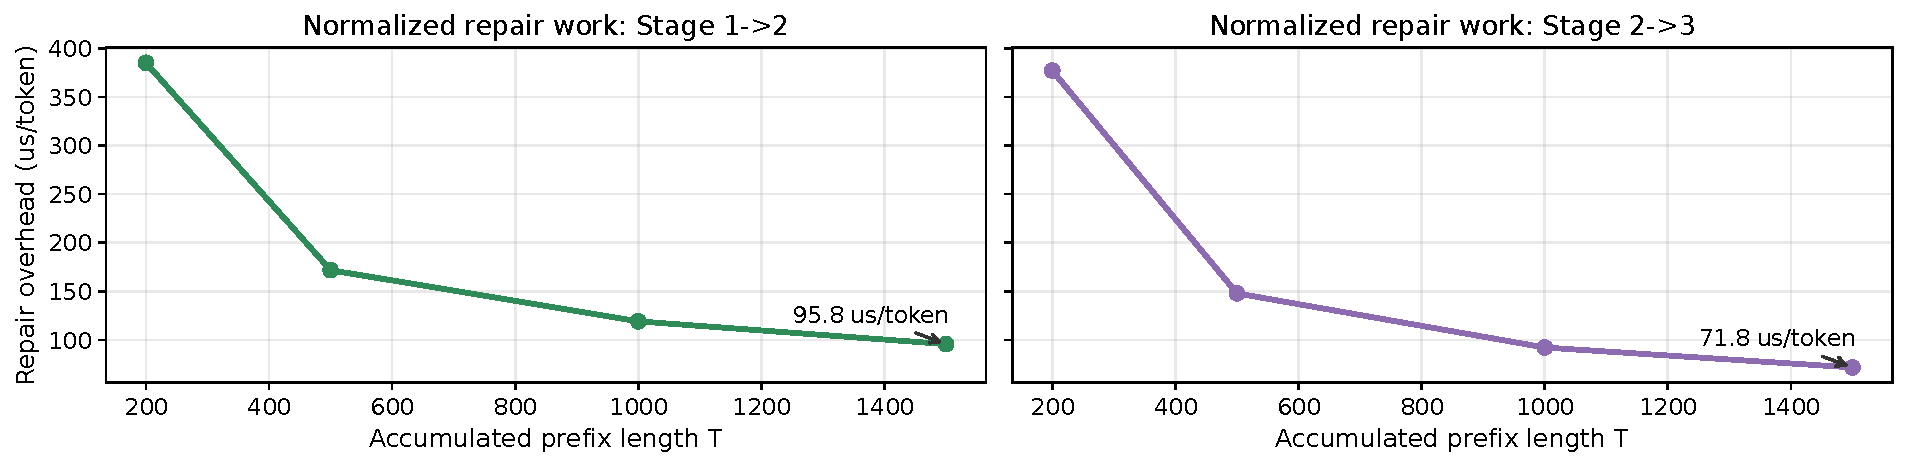
\includegraphics[width=0.96\textwidth]{figures/kv_repair_overhead_revision.pdf}
\caption{
Normalized repair overhead for the representative LLaMA-2-7B origin-first scaling sweep. As prefix length grows, the per-token repair work decreases because the fixed synchronization and boundary-local rematerialization cost is amortized over a longer cached context.
}
\label{fig:kv-repair-overhead-app}
\end{figure*}

\begin{table*}[t]
\centering
\small
\setlength{\tabcolsep}{4pt}
\renewcommand{\arraystretch}{0.95}
\caption{
Exact KV-repair summary. \(\Delta\)PPL is measured relative to \textit{Oracle-Recompute} on the newly appended span. TTFT reduction is measured against \textit{Full-Reset} on the first post-promotion request at the longest tested prefix. Models are ordered consistently as LLaMA-2-7B, Falcon-7B, Gemma-7B, and LLaMA-2-13B.
}
\label{tab:kv-repair-summary-appendix}
\begin{tabular}{lrrrrcc}
\toprule
Model
& \makecell{Repair\\\(\Delta\)PPL on \(B\)}
& \makecell{Stale\\\(\Delta\)PPL on \(B\)}
& \makecell{Repair\\\(\Delta\)PPL on \(C\)}
& \makecell{Stale\\\(\Delta\)PPL on \(C\)}
& \makecell{TTFT reduction @ \(T_{\max}\)\\(Stage~\(1\!\rightarrow\!2\) / Stage~\(2\!\rightarrow\!3\), ms)}
& \makecell{Repair overhead @ \(T_{\max}\)\\(Stage~\(1\!\rightarrow\!2\) / Stage~\(2\!\rightarrow\!3\), \(\mu\)s/token)} \\
\midrule
LLaMA-2-7B
& \(-0.17\)
& \(+1.74\)
& \(+0.02\)
& \(+3.87\)
& 171.0 / 174.1
& 95.8 / 71.8 \\
Falcon-7B
& \(-0.50\)
& \(+1.08\)
& \(+0.60\)
& \(+6.79\)
& 173.3 / 180.6
& 89.6 / 78.5 \\
Gemma-7B
& \(+0.08\)
& \(+2.76\)
& \(+0.12\)
& \(+4.91\)
& 204.6 / 207.8
& 214.0 / 199.1 \\
LLaMA-2-13B
& \(-0.12\)
& \(+1.03\)
& \(+0.10\)
& \(+1.43\)
& 321.7 / 326.6
& 137.4 / 109.1 \\
\bottomrule
\end{tabular}
\end{table*}

\paragraph{Token-count note.}
The longest realized prefix is \(T_{\max}{=}1500\) for both LLaMA models, \(1487\) for Falcon-7B, and \(1483\) for Gemma-7B because the realized token count follows the model-specific tokenizer.
